\documentclass{article}

\title{Lab 4 - Edge and line detection\\
	\large{Computer Vision}}
\author{Alberto Pasqualetto, 2121718}
\date{14 April 2024}

\usepackage[english]{babel}
% \usepackage{parskip}
\usepackage{float}
\usepackage{graphicx}
\usepackage{caption}
\usepackage{subcaption}
\graphicspath{ {./img/} }
\usepackage{cleveref}
\usepackage{xcolor}


% \newcommand{\mV}{\,\mathrm{mV}}


\begin{document}
\maketitle

The original base image is shown in figure \ref{fig:original}.
\begin{figure}[H]
	\centering
	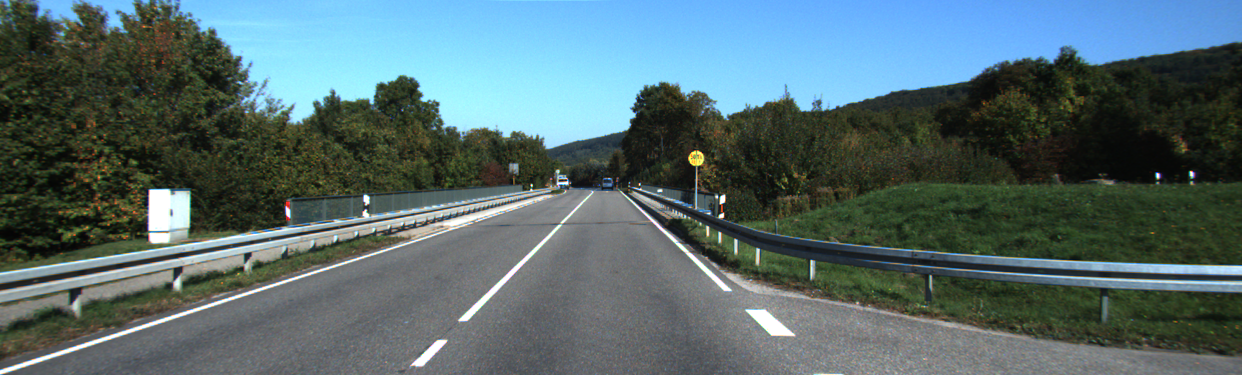
\includegraphics[width=0.9\textwidth]{../street_scene.png}
	\caption{Original image}
	\label{fig:original}
\end{figure}

\section*{Task 1}
In task 1 the aim is to use the OpenCV's Canny filter in order to detect edges in an image and test it using different values of its threshold selected by a trackbar directly in the image's window as seen in image \ref{fig:canny_trackbar}. The trackbar selects the lower threshold, instead the higher threshold is set to be 3 times the lower one as suggested by the OpenCV documentation.

The results of Canny filter with different thresholds are shown in figure \ref{fig:canny_results}: raising thresholds, less edges, the main ones, are detected.

\begin{figure}[H]
	\centering
	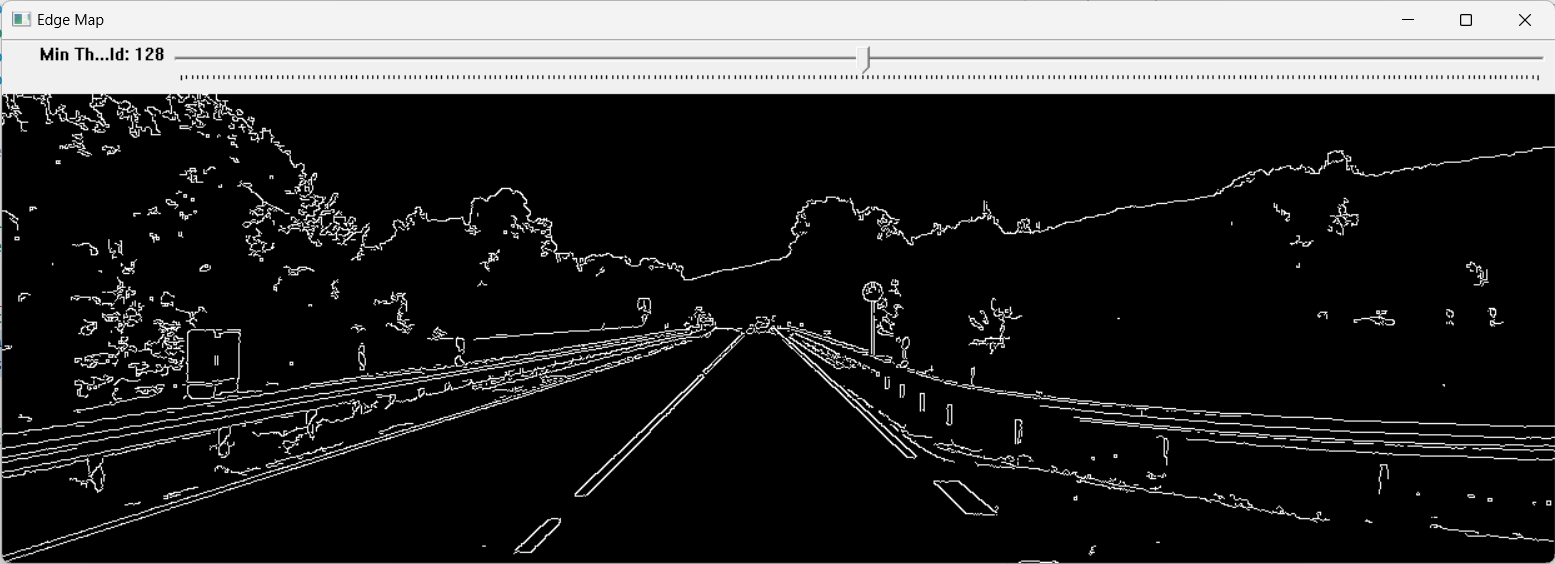
\includegraphics[width=0.9\textwidth]{street_scene_cannyTrackbarWindow.png}
	\caption{Window with trackbar for Canny min threshold selection}
	\label{fig:canny_trackbar}
\end{figure}

\begin{figure}[H]
	\centering
	\begin{subfigure}{0.49\textwidth}
		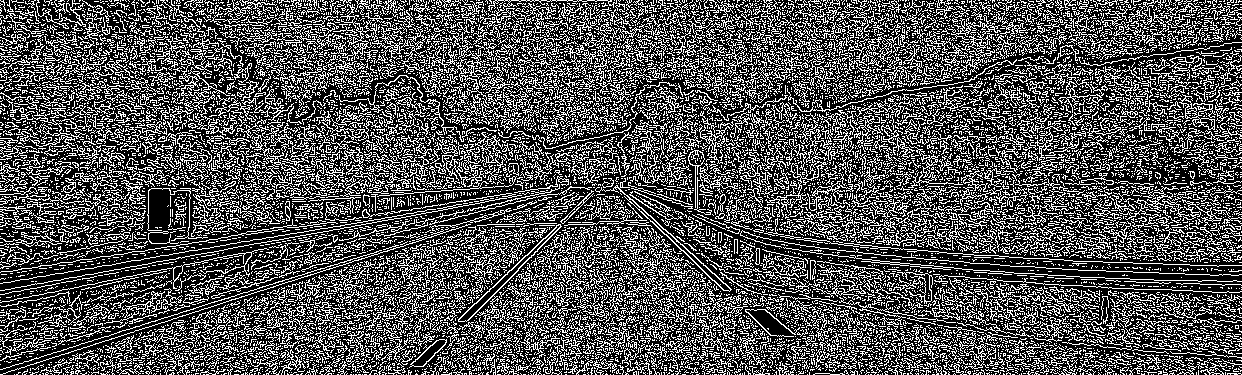
\includegraphics[width=\textwidth]{street_scene_thresholdMin1Max3.png}
		\caption{Thresholds 1 and 3}
	\end{subfigure}
	\hfill
	\begin{subfigure}{0.49\textwidth}
		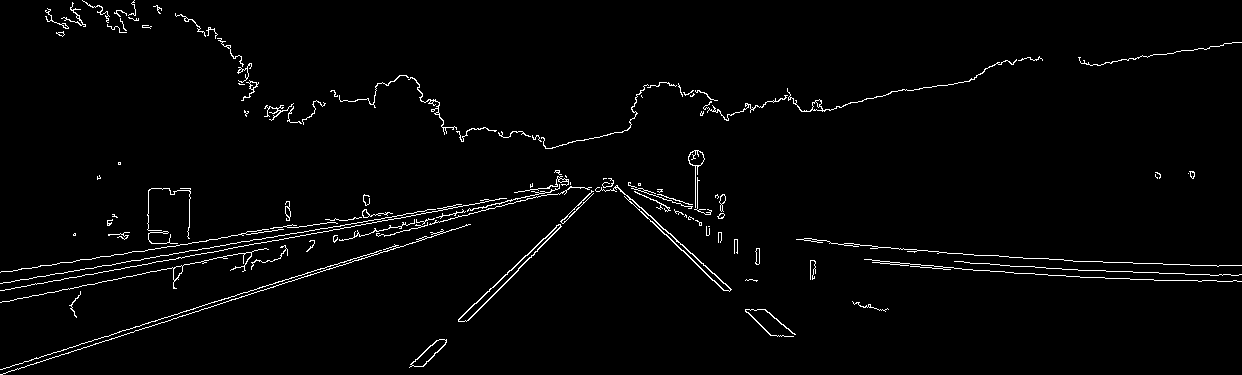
\includegraphics[width=\textwidth]{street_scene_thresholdMin255Max765.png}
		\caption{Thresholds 255 and 765}
	\end{subfigure}
	\caption{Canny filter results with different thresholds}
	\label{fig:canny_results}
\end{figure}


\section*{Task 2}
In task 2 it is required to detect the white lines on the road without using the Hough transform.

In order to do that first of all a mask for white color is created using the function \texttt{cv::inRange} and a very limited range.
Starting from the mask, 2 points for each white line (the middle and the right ones) on the image are found by looking for the first white pixel starting from the middle of the image going left (for left line) and right (for right line) at 2 different heights (4/6 and 5/6 of the image height, selected empirically).

Finally the equation of the line is calculated using the 2 points found for each line and both lines are drawn on the image in red as shown in figure \ref{fig:lines_noHough}.

\begin{figure}[H]
	\centering
	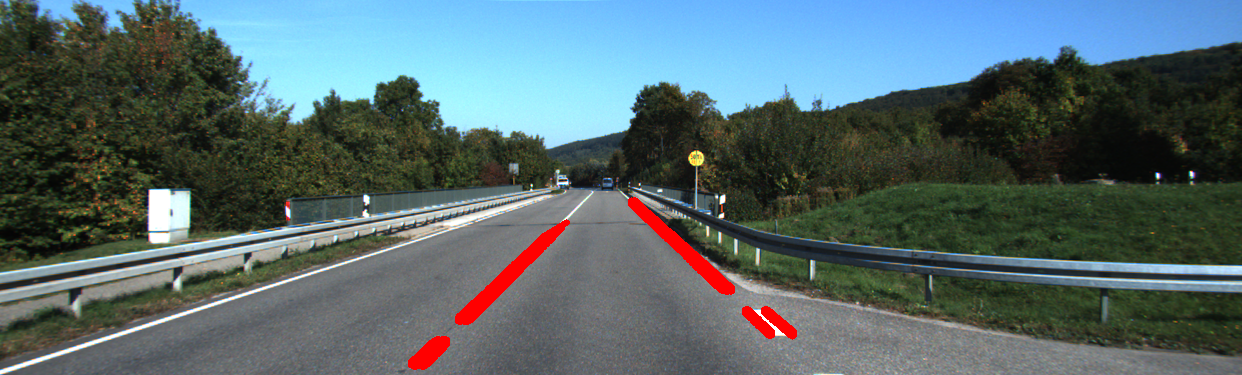
\includegraphics[width=0.9\textwidth]{street_scene_linesNoHough.png}
	\caption{Lines detected without Hough transform}
	\label{fig:lines_noHough}
\end{figure}



\section*{Task 3}
In task 3 it is required to detect the white lines on the road (middle and right one) using the Hough transform and then color in red the road between the lines.

In order to accomplish this task, the following steps are taken:
\begin{enumerate}
	\item The image is converted to grayscale.
	\item The Canny filter is applied to detect edges using empirically chosen thresholds (100 and 255).
	\item Hough transform is applied to detect lines in the image using the OpenCV function \texttt{cv::HoughLines} using the empirical threshold 150.
	\item Keep only one line that have a slope near $\frac{1}{4} \pi$ and one line with slope near $\frac{3}{4} \pi$ to filter out horizontal and vertical lines and remain with no more than 2 lines. (Selected slopes are decided by visualizing the original image and confirmed by testing different values).
	\item Draw the lines over the image of Canny filter like in figure \ref{fig:2lines_Hough}.
	\item Find the perspective vanishing point which is the intersection of the 2 lines at the top of the road.
	\item Find a point at the bottom of each line by picking the red pixels drawn in figure \ref{fig:2lines_Hough}.

	In order to ensure that the lines' pixels are present and exactly red (RGB(255, 0, 0)) at the last row of the image, the lines were drawn in the previous step using \texttt{lineType=cv::LINE\_8}, without antialiasing.
	\item Draw a red-filled polygon which connects the 3 points found above (realistically the points are more than 3 since those found from the bottom of lines can be more than one each since lines can be made of more than one pixel in each row, but this is not a problem for polygon drawing).
\end{enumerate}

The result is shown in figure \ref{fig:road_red_Hough}.

\begin{figure}[h]
	\centering
	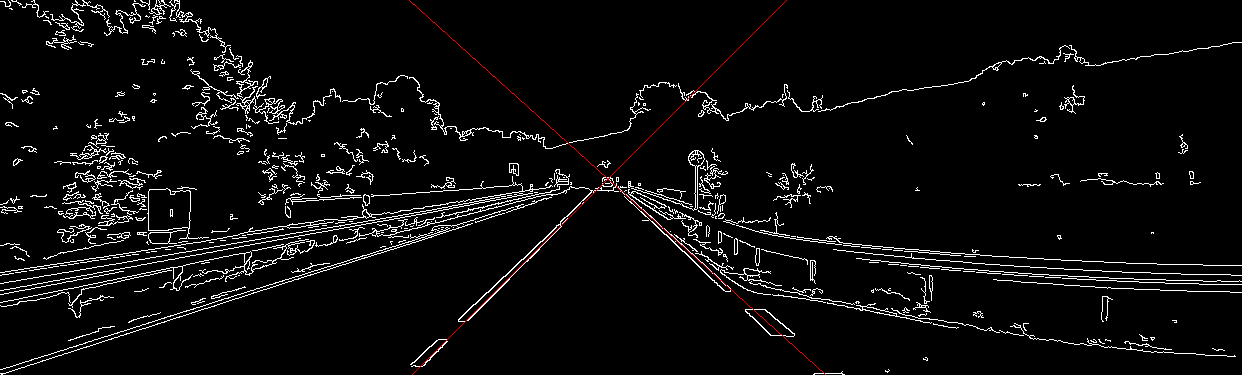
\includegraphics[width=0.9\textwidth]{street_scene_Hough2Lines.png}
	\caption{Lines detected with Hough transform}
	\label{fig:2lines_Hough}
\end{figure}

\begin{figure}[H]
	\centering
	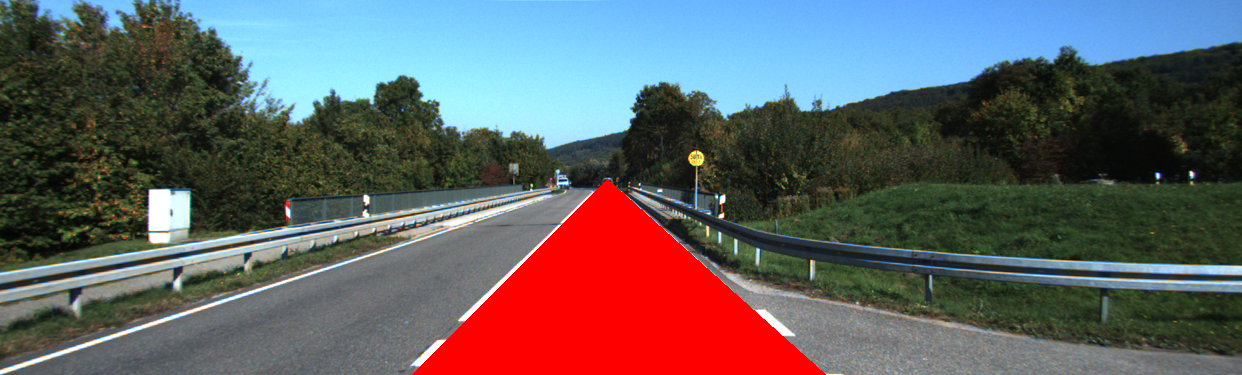
\includegraphics[width=0.9\textwidth]{street_scene_HoughRoadRed.png}
	\caption{Road colored in red between the lines detected with Hough transform}
	\label{fig:road_red_Hough}
\end{figure}


\section*{Task 4}
This task requires to detect the road sign using the Hough circular transform.
First of all a gaussian blur is applied on the image to reduce noise and result in less false circles detected.
Then the Hough circular transform is applied through the \texttt{cv::HoughCircles()} function which is called with the following parameters: \texttt{dp=2, method=cv::HOUGH\_GRADIENT, minDist=10, param1=200, param2=30, minRadius=7, maxRadius=12}.
Parameters were found empirically by testing different values. Specifically the targeted radius of the sign is about 8 pixels, so the min and max radius are set to 7 and 12 respectively in order to pick it and exclude the other circles.
Results can be observed in figure \ref{fig:sign_Hough}.

\begin{figure}[H]
	\centering
	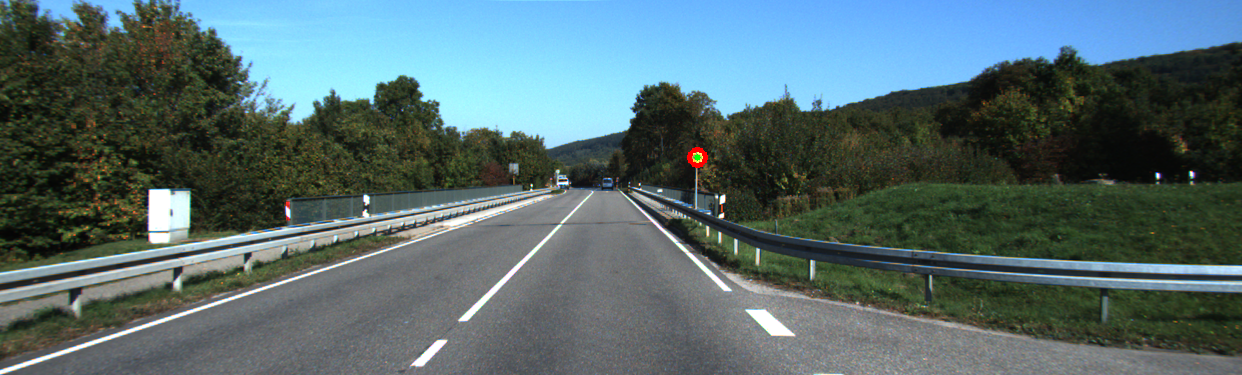
\includegraphics[width=0.9\textwidth]{street_scene_HoughSign.png}
	\caption{Road sign detected with Hough circular transform}
	\label{fig:sign_Hough}
\end{figure}




\end{document}
